\chapter{Downloading and Installing Salome}
\thispagestyle{empty}
\label{sec:chap5}
\newcommand{\LocCHfivefig}{\Origin/CHAPTERS/chap5/figures}

Salome is a Free and Open Source  CAD (Computer Aided Drawing), Meshing and Visualization Software for Numerical simulation. 
We can Create/modify, import/export (IGES, STEP, BREP), repair/clean CAD models and Mesh CAD models, edit mesh, check mesh quality, 
import/export mesh (MED, UNV, DAT, STL) using Salome. In this chapter we will learn how to download and intall Salome in any Operating system.

\section{Download Salome}

Open your browser and in the address bar type the url given below, \newline

\centering \textbf{www.salome-platform.org} \newline

\flushleft To Download Salome the user needs to create a account on the salome site. To do this on the left hand side of the salome screen website
scroll down to the bottom of the \textbf{Navigation} bar, Fig \ref{navi}, where you can see the new user option. Click on it and enter the required
personal details. \newline
\flushleft After you enter the details click on the register button at the bottom as shown in, Fig \ref{details}. Once done you will be directed 
to a screen showing that you have been registered. This also states thatv once you have done with registration you have to login to your email. Now 
open the mail sent by Salome and click on the link shown in Fig, \ref{link}. This link will direct you to a window where you need to set your password
for your Salome account. Enter the password and confirm it and press set my password button, Fig \ref{pass}. After this it will direct you to a window
which says your password has been set successfully. You may now login with your username and password. \newline

\flushleft In the Navigation bar click on Downloads after which you will be directed to a page which will show various bianaries for various Linux
distributions. You can choose according to your Operating System and 32/64 bit size. Since in this book we are working on a 64 bit platform we
will download Linux Debian 7 64-bits or Ubuntu 14.04 64-bits binary, Fig \ref{binary}. Click on it and Save the file. Since the file size is big it will take some time to download.
After this scroll down to Universal Binaries and click on the \textbf{Linux 64-bits} to download it. Note that 32-bit version of binaries are no
more supported for the latest version of Salome.

\begin{figure}[h]  
\centering
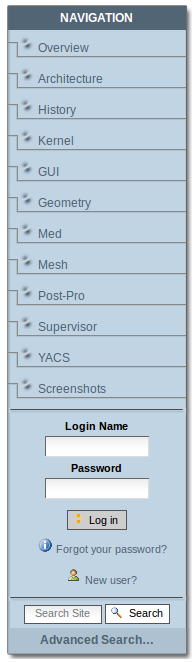
\includegraphics[scale=0.3]{\LocCHfivefig/navi.png}
\caption{Navigation Bar}
\label{navi}
\end{figure}

\begin{figure}[h]  
\centering
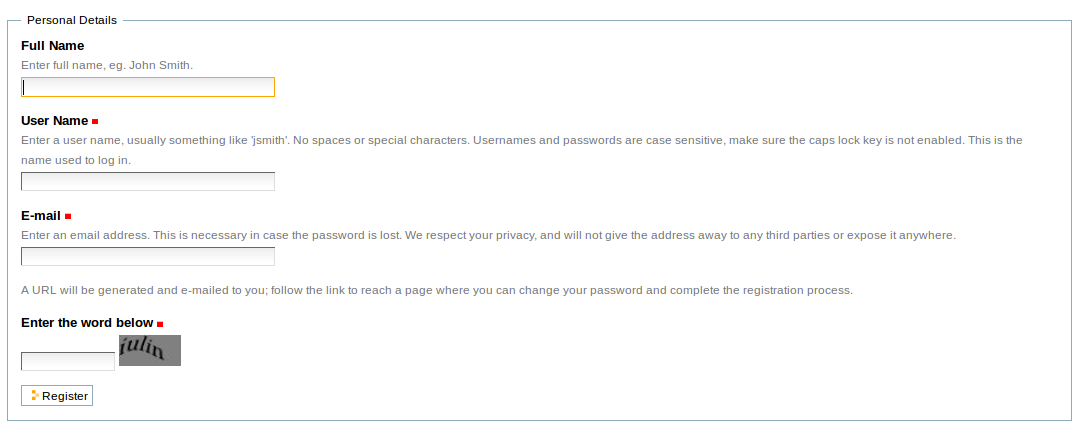
\includegraphics[scale=0.32]{\LocCHfivefig/details.png}
\caption{User Details}
\label{details}
\end{figure}

\begin{figure}[h]  
\centering
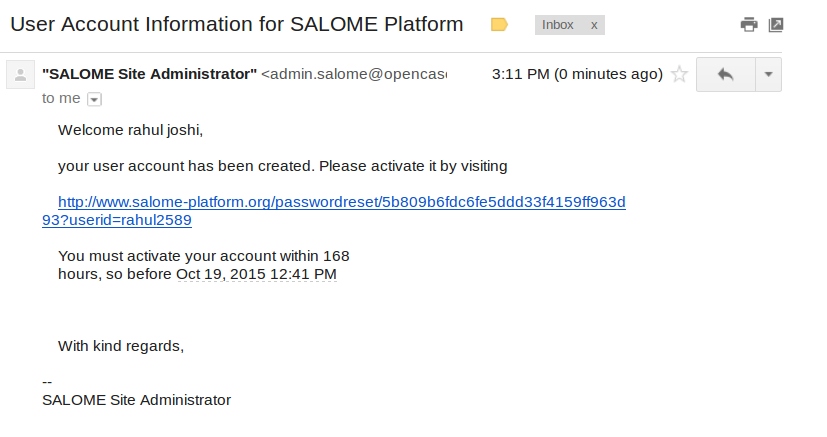
\includegraphics[scale=0.35]{\LocCHfivefig/link.png}
\caption{Salome Link}
\label{link}
\end{figure}

\begin{figure}[h]  
\centering
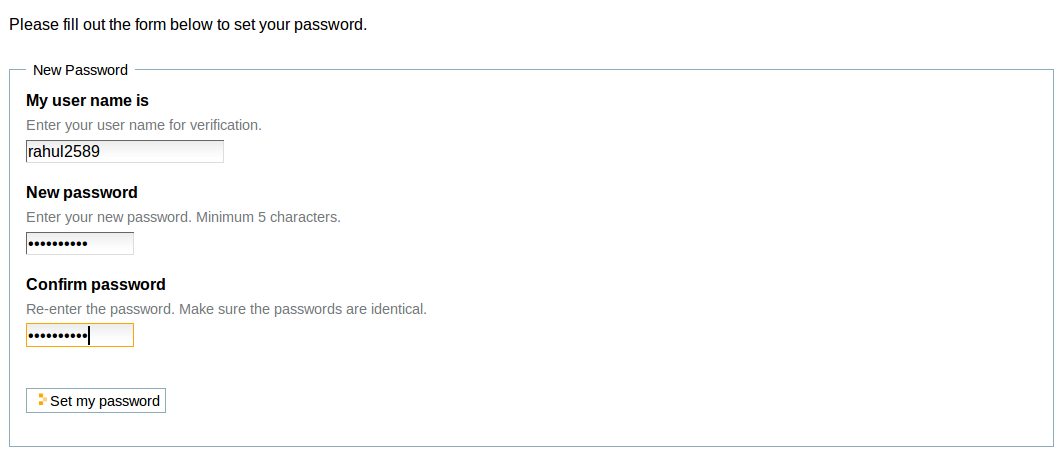
\includegraphics[scale=0.35]{\LocCHfivefig/pass.png}
\caption{Enter Password}
\label{pass}
\end{figure}

\begin{figure}[h]  
\centering
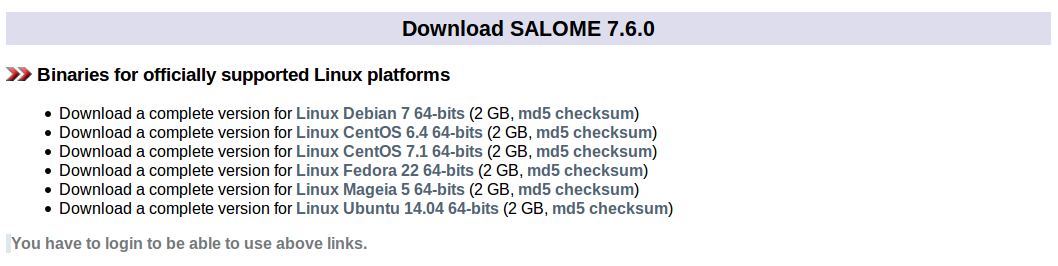
\includegraphics[scale=0.35]{\LocCHfivefig/binary.png}
\caption{Salome Linux Debain 7 64 bit binary}
\label{binary}
\end{figure}

\begin{figure}[h]  
\centering
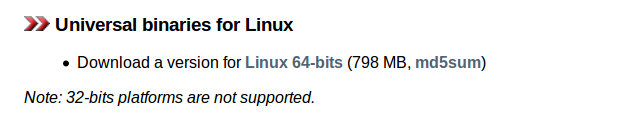
\includegraphics[scale=0.45]{\LocCHfivefig/universal.png}
\caption{Universal Binaries}
\label{univ}
\end{figure}

\section{Installing Salome}

The downloaded files are saved in the Download folder. Open the Download folder in your system and check for both the tar file and a self-extracting file.
Copy these two files and in your home folder create a new folder by the name Salome and paste these two files inside it, Fig \ref{download}.


